\documentclass[]{article}

% Imported Packages
%------------------------------------------------------------------------------
\usepackage{amssymb}
\usepackage{amstext}
\usepackage{amsthm}
\usepackage{amsmath}
\usepackage{enumerate}
\usepackage{fancyhdr}
\usepackage[margin=1in]{geometry}
\usepackage{graphicx}
\usepackage{extarrows}
\usepackage{setspace}
%------------------------------------------------------------------------------

% Header and Footer
%------------------------------------------------------------------------------
\pagestyle{plain}  
\renewcommand\headrulewidth{0.4pt}                                      
\renewcommand\footrulewidth{0.4pt}                                    
%------------------------------------------------------------------------------

% Title Details
%------------------------------------------------------------------------------
\title{Deliverable \#3 Template}
\author{SE 3A04: Software Design II -- Large System Design}
\date{}                               
%------------------------------------------------------------------------------

% Document
%------------------------------------------------------------------------------
\begin{document}

\maketitle	

\section{Introduction}
\label{sec:introduction}
% Begin Section

This section should provide a brief overview of the entire document.

\subsection{Purpose}
\label{sub:purpose}
% Begin SubSection
\begin{enumerate}[a)]
    \item The purpose of this document is to provide an exhaustive depiction of the Secure Chat Application's architecture through detailed design artifacts. It includes state chart diagrams for controller classes, sequence diagrams for each application use case, and a comprehensive class diagram capturing the entirety of the application's design.
    \item This document targets a wide range of internal stakeholders, including project managers, developers, domain experts, and team members, facilitating a deeper understanding of the application's design and functionality. It is recommended that Deliverables 1 and 2 be reviewed prior to engaging with this document, as they lay the foundation for the architectural and requirement specifications covered herein.
\end{enumerate}
% End SubSection

\subsection{System Description}
\label{sub:system_description}
% Begin SubSection
\begin{enumerate}[a)]
    \item The Secure Chat Application is conceived to establish secure communication channels among employees within an organization, utilizing company-issued Android devices. At its core, the application features a Key Distribution Centre (KDC) for key management, mediated authentication protocols for secure access, and employs robust symmetric-key cryptography for message encryption and decryption. Additionally, it maintains a secure log of chat histories on the server, addressing the organization's requirements for confidentiality and integrity in internal communications. This document extends the system overview presented in Deliverable 2, providing detailed design perspectives essential for the application's development.
\end{enumerate}
% End SubSection

\subsection{Overview}
\label{sub:overview}
% Begin SubSection
\begin{enumerate}[a)]
    \item Organized systematically by diagram type, this document is structured to facilitate easy navigation and understanding. Section 2 presents the state chart diagrams for controller classes, illustrating the application's behavior in various states.
    \item Section 3 delves into the sequence diagrams for each use case, showcasing the interactions between different system components. Section 4 concludes with a detailed Unified Modeling Language (UML) class diagram, offering a holistic view of the application's design structure. Together, these sections compose a comprehensive blueprint for the Secure Chat Application, guiding the development process towards successful implementation.
\end{enumerate}
% End SubSection

% End Section


\section{State Charts for Controller Classes}
\label{sec:state_charts_for_controller_classes}
% Begin Section
This section should provide a state chart for each controller class for your application.

\begin{figure}[H]
	\centering
	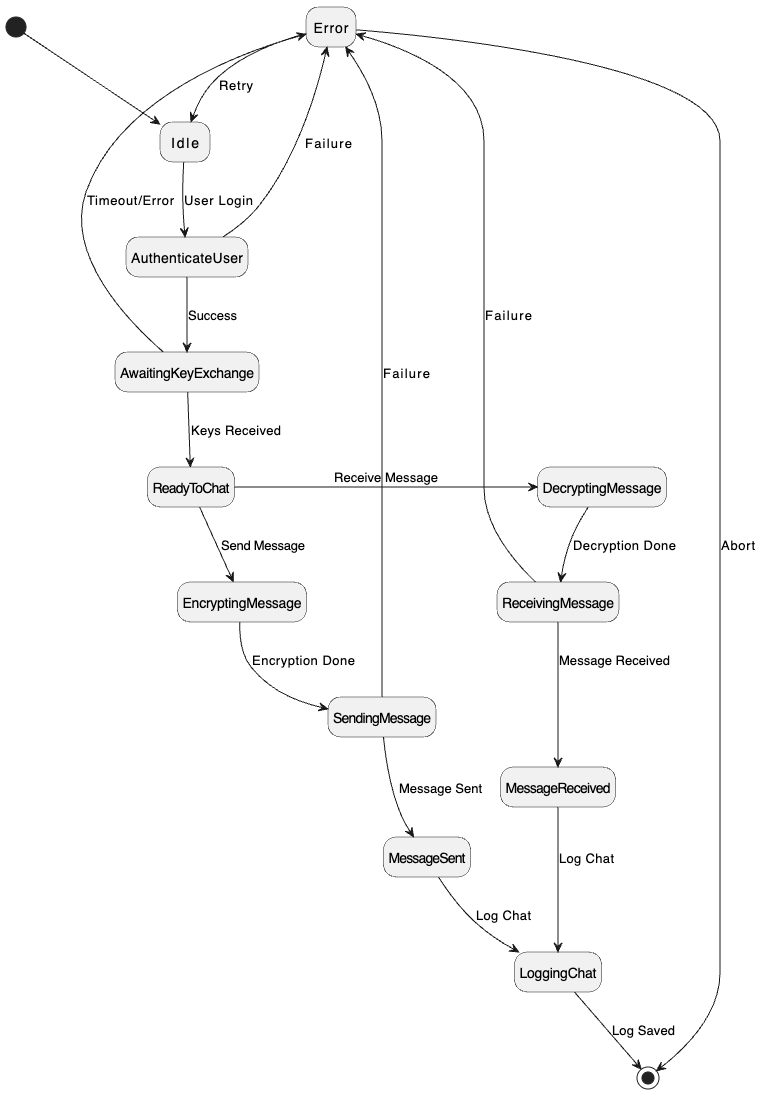
\includegraphics[width=1\textwidth]{chat_controller.drawio.png}
	\caption{State Chart for Chat Controller}
\end{figure}
% End Section

\section{Sequence Diagrams}
\label{sec:sequence_diagrams}
% Begin Section
This section should provide a sequence diagram for each use case of your application.
% End Section

\section{Detailed Class Diagram}
\label{sec:detailed_class_diagram}
% Begin Section
This section should provide a detailed class diagram for your application.
% End Section

\appendix
\section{Division of Labour}
\label{sec:division_of_labour}
% Begin Section
Include a Division of Labour sheet which indicates the contributions of each team member. This sheet must be signed by all team members.
% End Section

\newpage
\section*{IMPORTANT NOTES}
\begin{itemize}
	\item You do \underline{NOT} need to provide a text explanation of each diagram; the diagram should speak for itself
	\item Please document any non-standard notations that you may have used
	\begin{itemize}
		\item \emph{Rule of Thumb}: if you feel there is any doubt surrounding the meaning of your notations, document them
	\end{itemize}
	\item Some diagrams may be difficult to fit into one page
	\begin{itemize}
		\item It is OK if the text is small but please ensure that it is readable when printed
		\item If you need to break a diagram onto multiple pages, please adopt a system of doing so and throughly explain how it can be reconnected from one page to the next; if you are unsure about this, please ask me
	\end{itemize}
	\item Please submit the latest version of Deliverable 1 and Deliverable 2 with Deliverable 3
	\begin{itemize}
		\item They do not have to be a freshly printed versions; the latest marked versions are OK
	\end{itemize}
	\item If you do \underline{NOT} have a Division of Labour sheet, your deliverable will \underline{NOT} be marked
\end{itemize}


\end{document}
%------------------------------------------------------------------------------